\documentclass[../paper.tex]{subfiles}
\begin{document}
In physics, particles are sometimes represented as point-particles \cite{PointParticle}. Particles from which the size, shape and structure do not matter in a specific context can be represented as point-particles. Visually, if you would zoom out enough on any particle, it would appear to be a point, rather than a particle with multiple dimensions (such as shape). In String Theory, the point-like particles of particle physics (shown in \ref{Elementary Particles}), are represented as one-dimensional strings \cite{StringTheory}. One of the vibrational states of the string is Graviton. Graviton is a quantum mechanical particle that has gravitational force and thus, String Theory can be described as a theory for quantum gravity. String Theory in it's complete form would potentially be a unified description of gravity and particle physics. This makes the theory an option for a "Theory of Everything". A Theory of Everything would be a theoretical framework that links and explains all physical aspects of the universe \cite{TheoryOfEverything}. A lot of particles and forces are already known by mankind, but some new ones might show up in String Theory as well. In order to make any claims on what new particles and forces might be predicted by String Theory, the theory needs to be verified first, by the parts we already know. Complete verification will not be able in this way, but it's good approach to find in what direction we must be searching. If this verification fails, String Theory will not be a unified description of the universe. 

\begin{figure}[!htb]
\centering
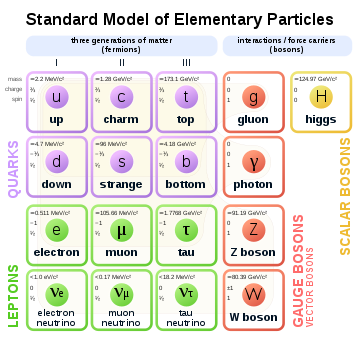
\includegraphics[scale = 0.5]{String Theory/ElementaryParticles.png}
\caption{Elementary Particles}
\label{Elementary Particles}
\end{figure}

\end{document}